\section{An Iterative Approach to Data Analysis and
Modeling}



\begin{frame}
 \frametitle{Iterative Approach}
 \begin{itemize}
   \item Model formulation stage
   \item Fitting
   \item Diagnostic checking - the data and model must be consistent with one another
before additional inferences can be made.
 \end{itemize}

  \begin{figure}[htp]
    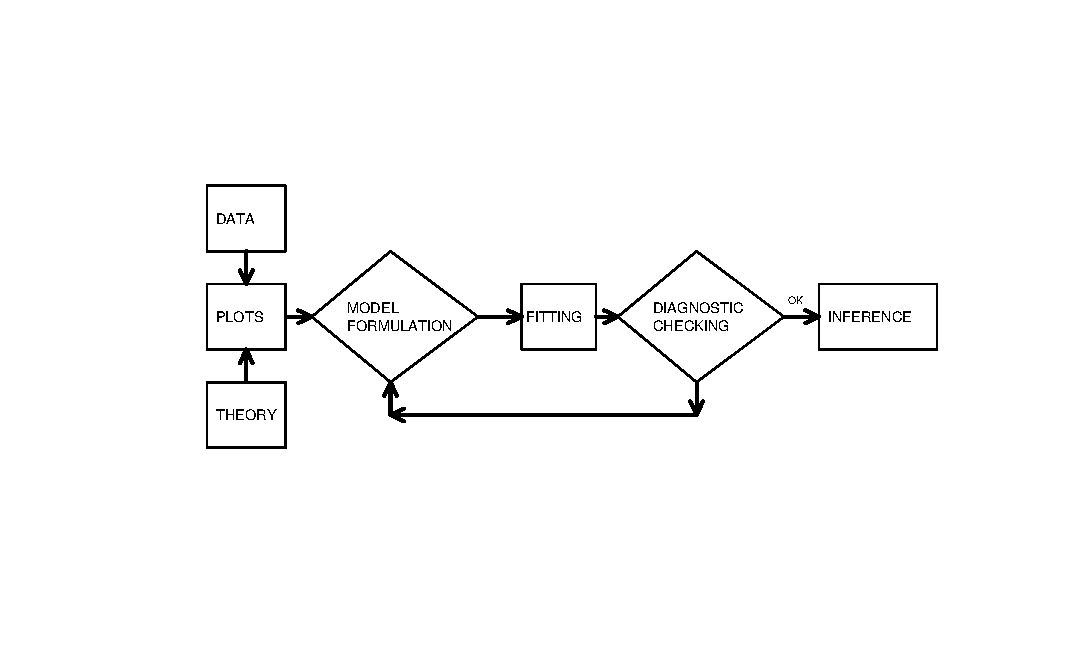
\includegraphics[width=1\textwidth,angle=0,scale=1]{Chapter5/FigJed5_1.ps}
  \end{figure}
\end{frame}


\section{Automatic Variable Selection Procedures}

\begin{frame}%[shrink=10]
 \frametitle{Many possible models}
\begin{table}[h]
\scalefont{0.8}

\caption{ Sixteen Possible Models}
\begin{tabular}{llll}
\hline
E $y=\beta _{0}$ &  &  & 1 model with no  \\
&  &  & \ \ variables \\
E $y=\beta _{0}+\beta _{1}x_{i},$ & $i=$ & $1,2,3,4$ & 4 models with
one
 \\
&  &  & \ \ variable \\
E $y=\beta _{0}+\beta _{1}x_{i}+\beta _{2}x_{j},$ & $(i,j)=$ & $%
(1,2),(1,3),(1,4),$ & 6 models with two  \\
&  & $(2,3),(2,4),(3,4)$ & \ \ variables \\
E $y=\beta _{0}+\beta _{1}x_{1}+\beta _{2}x_{j}$ & $(i,j,k)=$ & $%
(1,2,3),(1,2,4),$ & 4 models with three  \\
$\ \ \ \ \ \ \ \ +\beta _{3}x_{k},$ &  & $(1,3,4),(2,3,4)$ & \ \
variables
\\
E $y=\beta _{0}+\beta _{1}x_{1}+\beta _{2}x_{2}$ &  &  & 1 model
with all
\\
$\ \ \ \ \ \ \ \ +\beta _{3}x_{3}+\beta _{4}x_{4}$ &  &  & \ \ variables \\
\hline
\end{tabular}
\scalefont{1.25}
\end{table}
 \begin{itemize}%[<+->]
 \pause
   \item With $k$ explanatory variables, there are $2^k$ possible
   linear models
   \item There are infinitely many nonlinear ones!!
    \end{itemize}
\end{frame}


\begin{frame}%[shrink=2]
 \frametitle{Stepwise Regression Algorithm}
Suppose that the analyst has identified one variable as the
response, $y$, and $k$ potential explanatory variables, $x_1, x_2,
\ldots, x_k$.
 \begin{itemize}
\scalefont{0.8}

\item (i). Consider all possible regressions using one explanatory variable.
For each of the $k$ regressions, compute $t(b_1)$, the $t$-ratio for
the slope. Choose that variable with the largest $t$-ratio. If the
\textit{t}-ratio does not exceed a pre-specified $t$-value (such as
two), then do not choose any variables and halt the procedure.

\item (ii). Add a variable to the model from the previous step. The variable to enter
is the one that makes the largest significant contribution. To
determine the
size of contribution, use the absolute value of the variable's \textit{t}%
-ratio. To enter, the $t$-ratio must exceed a specified $t$-value in
absolute value.

\item (iii). Delete a variable to the model from the previous step. The variable to be
removed is the one that makes the smallest contribution. To
determine the size of contribution, use the absolute value of the
variable's $t$-ratio. To be removed, the $t$-ratio must be less than
a specified $t$-value in absolute value.

\item (iv). Repeat steps (ii) and (iii) until all possible additions and deletions are
performed.

\scalefont{1.25}
 \end{itemize}
\end{frame}


\begin{frame}%[shrink=10]
 \frametitle{Drawbacks of Stepwise Regression}
 \scalefont{0.8}
 \begin{itemize}

\item The procedure ``snoops'' through a large number of models and may
fit the data ``too well.''

\item There is no guarantee that the selected model is the best. The algorithm
does not consider models that are based on nonlinear combinations of
explanatory variables. It also ignores the presence of outliers and
high leverage points.

  \item In addition, the algorithm does not even search all $2^{k}$ possible
linear regressions.

  \item The algorithm uses one criterion, a \textit{t}-ratio, and does not
consider other criteria such as s, $R^{2}$, R, and so on.

  \item There is a sequence of significance tests involved. Thus, the
significance level that determines the \textit{t}-value is not
meaningful.

  \item By considering each variable separately, the algorithm does not take into
account the joint effect of independent variables.

  \item Purely automatic procedures may not take into account an investigator's
special knowledge.

    \end{itemize}
    \scalefont{1.25}
\end{frame}

\begin{frame}%[shrink=10]
 \frametitle{Variants of Stepwise Regression }
 \begin{itemize}
\item Forward selection. Add one variable at a time without trying
to delete variables.

\item Backwards selection. Start with the full model and delete one variable at
a time without trying to add variables.
\item Best regressions.
    \end{itemize}
\end{frame}

\begin{frame}[fragile]
 \frametitle{Data-Snooping in Stepwise Regression}
 \begin{itemize}
   \item Generate $y$ and $x_1 - x_{50}$ using a random number generator
  \item By design, there is no relation between $y$ and $x_1 - x_{50}$.
    \end{itemize}
    \scalefont{0.8}
\begin{alltt}
Minitab Ouptput
    MTB > step 'Y' using c2-c51

 STEPWISE REGRESSION OF  Y  ON 50 PREDICTORS, WITH N =  100
    STEP        1        2

CONSTANT-0.004371-0.021359
C49          0.25     0.25
T-RATIO      2.29     2.29
C51                  -0.24
T-RATIO              -2.18

S            1.07     1.05
R-SQ         5.06     9.50

 MORE? (YES, NO, SUBCOMMAND, OR HELP)
SUBC> n
\end{alltt}
\scalefont{1.25}

\end{frame}

\begin{frame}%[shrink=10]
 \frametitle{Automatic Variable Selection Procedures}
 \begin{itemize}
 \item Stepwise regression and best regressions are examples of
automatic variable selection procedures.
 \begin{itemize}
 \item These procedures are useful because they can
quickly search through several candidate models.
\item They ignore nonlinear alternatives as well as the effect of
outliers and high leverage points.
\item They  mechanize certain routine tasks.
\item Other so-called
``expert systems'' available in the market. For example, algorithms
are available that ``automatically'' handle unusual points such as
outliers and high leverage points.
    \end{itemize}
   \item A model suggested by automatic variable selection
procedures should be subject to the same careful diagnostic checking
procedures as a model arrived at by any other means.
    \end{itemize}
\end{frame}

\section{Residual Analysis}

\begin{frame}%[shrink=10]
 \frametitle{Residual Analysis}
 \begin{itemize}
   \item Role of residuals:  If the model formulation is correct, then residuals $\approx$ random errors.
 \item Four types of Patterns:
\begin{itemize}
   \item Unusually large residuals
   \item Residuals related to explanatory variables
\item Heteroscedastic residuals (Section 5.7)
\item Time patterns in residuals (start in Chapter 7)
\end{itemize}
\item Method of attack: Look for patterns in the residuals. Use this information to improve
the model specification.
    \end{itemize}
\end{frame}



\subsection{Residuals}

\begin{frame}%[shrink=10]
 \frametitle{Residuals}
 \begin{itemize}
   \item Standardized residual = residual divided by it's estimated standard error.
\item Use standardized residuals because:
 \begin{itemize}
   \item we can focus on relationships of interest
\item achieve carry-over of experience from one data set to another.
\end{itemize}
\item Using $e_i = y_{i}-\hat{y}_{i}$ as the $i$th residual, here are
three commonly used definitions:
\begin{equation*}
\text{(a) }\frac{e_i}{s},\text{ \ \ \ (b) }\frac{e_i}{s\sqrt{%
1-h_{ii}}}, \text { \  \   \   }\text{(c)
}\frac{e_i}{s_{(i)}\sqrt{1-h_{ii}}}\text{\ }.
\end{equation*}
\item First choice is simple
\item Second choice, from theory,  $\mathrm{Var}(e_i)=\sigma ^{2}(1-h_{ii}).$
Here, $h_{ii}$ is the $i$th leverage. It is calculated based on
values of the explanatory variables and will be defined in Section
5.4.1.
\item Third choice is termed ``studentized residuals''. Idea: numerator is
independent of the denominator.
    \end{itemize}
\end{frame}

\subsection{Using Residuals to Identify Outliers}


\begin{frame}%[shrink=10]
 \frametitle{Outliers}
 \begin{itemize}
   \item  An outlier is an observation that is not well fit by the model; these
are observations where the residual is unusually large.
 \item Unusual means what?  Many packages mark a point if the |standardized residual| > 2.
  \item Options for handling outliers
 \begin{itemize}
   \item  Ignore them in the analysis but be sure to discuss their
effects.
\item  Delete them from the data set (but be sure to discuss their
effects).
\item  Create a binary variable to indicator their presence. (This
will increase your $R^2$!)
    \end{itemize}
    \end{itemize}
\end{frame}

\subsection{Using Residuals to Select Explanatory
Variables}

\begin{frame}%[shrink=10]
 \frametitle{Using Residuals to Select Explanatory
Variables}
 \begin{itemize}
   \item Residual analysis can help identify
additional explanatory variables that may be used to improve the
formulation of the model.
 \begin{itemize}
   \item If the model is correct, then residuals should
resemble random errors and contain no discernible patterns.
\item Thus,
when comparing residuals to explanatory variables, we do not expect
any relationships.
\item If we do detect a relationship, then this
suggests the need to control for this additional variable.
   \end{itemize}
\item Ways of detecting relationships.
 \begin{itemize}

 \item Calculate summary statistics and display the distribution of
(standardized) residuals to identify outliers.

\item  Calculate the correlation between the (standardized) residuals and
additional explanatory variables to search for linear relationships.

\item  Create scatter plots between the (standardized) residuals and additional
explanatory variables to search for nonlinear relationships.

    \end{itemize}
    \end{itemize}
\end{frame}

\begin{frame}[shrink=2]
 \frametitle{Example. Stock Liquidity}
 \begin{itemize}
   \item Investors want high expected returns and low volatility.
   Sometimes, they also want to receive income from investments
   periodically (dividends).
   \item Investors also wish to be able to sell investments quickly,
   known as ``liquidity.''
  \item This study has $n=126$ companies.
  \item For the trading activity variables, we examine
\begin{itemize}
\item the three months total trading volume (VOLUME, in millions of shares),
\item the three months total number of transactions (NTRAN), and
\item the average time between transactions (AVGT, measured in minutes).
\end{itemize}
\item  For the firm size variables, we use the
\begin{itemize}
\item opening stock price on January 2, 1985 (PRICE),
\item  the number of outstanding shares on December 31, 1984 (SHARE, in millions of shares), and
\item  the market equity value (VALUE, in billions of dollars) obtained by taking the product of PRICE and SHARE.
\end{itemize}
    \end{itemize}
\end{frame}

\begin{frame}%[shrink=10]
 \frametitle{Example. Stock Liquidity}
\begin{table}[h]
\scalefont{0.9}

\caption{ Summary Statistics of the Stock Liquidity Variables}

\begin{tabular}{cccccc}
\hline
& Mean & Median & Standard & Minimum & Maximum \\
&  &  & deviation &  &  \\ \hline \multicolumn{1}{l}{VOLUME} &
\multicolumn{1}{r}{$13.423$} & \multicolumn{1}{r}{$11.556$} &
\multicolumn{1}{r}{$10.632$} &
\multicolumn{1}{r}{$0.658$} & \multicolumn{1}{r}{$64.572$} \\
\multicolumn{1}{l}{AVGT} & \multicolumn{1}{r}{$5.441$} & \multicolumn{1}{r}{$%
4.284$} & \multicolumn{1}{r}{$3.853$} & \multicolumn{1}{r}{$0.590$}
&
\multicolumn{1}{r}{$20.772$} \\
\multicolumn{1}{l}{NTRAN} & \multicolumn{1}{r}{$6436$} & \multicolumn{1}{r}{$%
5071$} & \multicolumn{1}{r}{$5310$} & \multicolumn{1}{r}{$999$} &
\multicolumn{1}{r}{$36420$} \\
\multicolumn{1}{l}{PRICE} & \multicolumn{1}{r}{$38.80$} & \multicolumn{1}{r}{%
$34.37$} & \multicolumn{1}{r}{$21.37$} & \multicolumn{1}{r}{$9.12$}
&
\multicolumn{1}{r}{$122.37$} \\
\multicolumn{1}{l}{SHARE} & \multicolumn{1}{r}{$94.7$} & \multicolumn{1}{r}{$%
53.8$} & \multicolumn{1}{r}{$115.1$} & \multicolumn{1}{r}{$6.7$} &
\multicolumn{1}{r}{$783.1$} \\
\multicolumn{1}{l}{VALUE} & \multicolumn{1}{r}{$4.116$} & \multicolumn{1}{r}{%
$2.065$} & \multicolumn{1}{r}{$8.157$} & \multicolumn{1}{r}{$0.115$}
&
\multicolumn{1}{r}{$75.437$} \\
\multicolumn{1}{l}{DEB\_EQ} & \multicolumn{1}{r}{$2.697$} &
\multicolumn{1}{r}{$1.105$} & \multicolumn{1}{r}{$6.509$} &
\multicolumn{1}{r}{$0.185$} & \multicolumn{1}{r}{$53.628$} \\ \hline
\end{tabular}

\textit{Source: Francis Emory Fitch, Inc., Standard \& Poor's
Compustat, and University of Chicago's Center for Research on
Security Prices.}

\scalefont{1.1111}
\end{table}
\end{frame}

\begin{frame}%[shrink=10]
 \frametitle{Example. Stock Liquidity}
 \begin{table}[h]
\scalefont{0.9}

\caption{\label{T5:LiquidCorr} Correlation Matrix of the Stock
Liquidity}
\begin{tabular}{lrrrrrrr}
\hline & AVGT & NTRAN & PRICE & SHARE & VALUE & DEB\_EQ \\ \hline
\multicolumn{1}{l}{NTRAN} & $-0.668$ &  &  &  &  &  \\
\multicolumn{1}{l}{PRICE} & $-0.128$ & $0.190$ &  &  &  &  \\
\multicolumn{1}{l}{SHARE} & $-0.429$ & $0.817$ & $0.177$ &  &  &  \\
\multicolumn{1}{l}{VALUE} & $-0.318$ & $0.760$ & $0.457$ & $0.829$ &  &  \\
\multicolumn{1}{l}{DEB\_EQ} & $0.094$ & $-0.092$ & $-0.038$ & $-0.077$ & $%
-0.077$ &  \\
\multicolumn{1}{l}{VOLUME} & $-0.674$ & $0.913$ & $0.168$ & $0.773$
& $0.702$ & $-0.052$ \\ \hline
\end{tabular}
\scalefont{1.1111}
\end{table}
 \begin{itemize}
   \item Liquidity variables, VOLUME, NTRAN and AVGT, are highly
   correlated

    \end{itemize}
\end{frame}

\begin{frame}%[shrink=10]
 \frametitle{Example. Stock Liquidity}
 \begin{itemize}
   \item A first regression yields
   \scalefont{0.8}
\begin{center}
\begin{tabular}{lccl}
  VOLUME & = & 1.65 & +0.00183 NTRAN \\
  std errors &  & (0.0018)  & (0.000074) \\
\end{tabular}
\end{center}
\scalefont{1.25}
 \item This also yields residuals. To see patterns in the residuals,
 here is a table of correlations:
 \begin{table}[h]
\scalefont{0.8}
\begin{tabular}{cccccc}
 \hline
& AVGT & PRICE & SHARE & VALUE & DEB\_EQ \\
RESID & -0.155 & -0.017 & 0.055 & 0.007 & 0.078 \\ \hline
\end{tabular}
\scalefont{1.25}
\end{table}

\item This suggests bring AVGT into the model, yielding the fit
 \scalefont{0.8}
\begin{center}
\begin{tabular}{lccll}
  VOLUME     & = & 4.41   & -0.322 AVGT & +0.00167 NTRAN \\
  std errors &   & (1.30) & (0.135)     & (0.000098)     \\
\end{tabular}
\end{center}
\scalefont{1.25}
\item  This table of correlations shows that there is not much going on with residuals from this model fit.
\begin{table}[h]
\scalefont{0.8}
\begin{tabular}{ccccc}
\hline
& PRICE & SHARE & VALUE & DEB\_EQ \\
RESID & -0.015 & 0.096 & 0.071 & 0.089 \\ \hline
\end{tabular}
 \scalefont{1.25}
\end{table}
    \end{itemize}
\end{frame}

\section{Influential Points}

\begin{frame}[shrink=2]
 \frametitle{Influential Points}
 \begin{itemize}
 \item Influential points are observations that potentially have a lot to say about a regression fit.
 They may have large residuals, high leverage, or both.
 \item We have seen that regression coefficients are weighted sums -
 not all observations are equal!
  \begin{itemize}
 \item Intuitively, observations that are ``far away'' in the
 $x$-space have greater influence.
 \item One can get a feel for influential observations by looking a
 summary statistics (mins, maxs) for each explanatory variable.
 \item However, this is not sufficient - see the graph below.
     \end{itemize}
   \item The ellipsoid
represents most of the data. The arrow marks an unusual point that
is not unusual for $x_1$ or $x_2$.
    \end{itemize}
\begin{figure}[htp]
  \begin{center}
    \includegraphics[width=1\textwidth,angle=270,scale=0.25]{Chapter5/Fig5_3.ps}
  \end{center}
\end{figure}
\end{frame}

\subsection{Leverage}


\begin{frame}[shrink=2]
 \frametitle{Leverage}
 \begin{itemize}
   \item The regression coefficients can be calculated
   as $\mathbf{b} = (\mathbf{X}^{\prime}\mathbf{X})^{-1}
   \mathbf{X}^{\prime}\mathbf{y}$.
   \item The vector of fitted values is
   $\mathbf{\widehat{y}}=\mathbf{Xb}$, so that $\mathbf{\widehat{y}}= \mathbf{X(X}^{\prime
}\mathbf{X)}^{-1}\mathbf{X}^{\prime }\mathbf{y}$
 \item \textbf{Hat Matrix}
  \begin{itemize}
   \item This suggests defining $\mathbf{H}=\mathbf{X(X}^{\prime }\mathbf{X)}^{-1}%
\mathbf{X}^{\prime }$.
 \item The matrix $\mathbf{H}$ \textit{projects} the vector of responses
 $\mathbf{y}$ onto the vector of fitted values $\mathbf{\widehat{y}}$.
 \item Think of $\mathbf{H}$ as the matrix that puts
the ``hat,'' or carat, on $\mathbf{y}$.
   \end{itemize}
 \item From the $i$th row of the vector equation $\mathbf{\widehat{y}=Hy}$, we have
\begin{equation*}
\widehat{y}_{i}=h_{i1}y_{1}+h_{i2}y_{2}+...+h_{ii}y_{i}+...+h_{in}y_{n}.
\end{equation*}
 \item Here, $h_{ij}$ is the number in the $i$th row and $j$th column of
$\mathbf{H} $. Because of this relationship, $h_{ii}$ is called the
``$i$th leverage.''
 \item Because $h_{ii}$ is the $i$th diagonal element of $%
\mathbf{H}$, a direct expression is
\begin{equation*}
h_{ii}=\mathbf{x}_{i}^{\prime }\mathbf{(X}^{\prime }\mathbf{X)}^{-1}\mathbf{x%
}_{i}
\end{equation*}
where $\mathbf{x}_{i}=(x_{i0},x_{i1},\ldots,x_{ik})^{\prime }$.
 \item Using matrix algebra, one can establish $ n^{-1}\leq h_{ii}\leq 1.$
    \end{itemize}

\end{frame}

\begin{frame}%[shrink=10]
 \frametitle{High Leverage Points}
 \begin{itemize}
   \item An observation is a high leverage point if the value of
   $h_{ii}$ is large.
 \begin{itemize}
   \item By algebra, the average leverage is $\bar{h}=\frac{1}{n}\sum_{i=1}^{n}h_{ii}=\frac{k+1}{n}.$
\item Some packages declare an observation to be a
\textit{high leverage point} if the leverage exceeds three times the
average, that is, if $h_{ii}>3(k+1)/n $.
  \end{itemize}
  \item Options for handling high leverage points (similar to
  outliers)
   \begin{itemize}
   \item  Ignore them in the analysis but be sure to discuss their
effects.
\item  Delete them from the data set (but be sure to discuss their
effects).
\item Choose another variable to represent the information.
\item  Use a nonlinear transformation of an explanatory variable.

    \end{itemize}
    \end{itemize}
\end{frame}

\subsection{Cook's Distance}


\begin{frame}[shrink=2]
 \frametitle{Cook's Distance}
 \begin{itemize}
   \item Another measure of ``influence.''  This measure considers both the explanatory and response
   variables.
   \item This distance, $D_{i}$, is defined as
\begin{equation*}
D_{i} =
\frac{\sum_{j=1}^{n}(\hat{y}_{j}-\hat{y}_{j(i)})^{2}}{(k+1)s^{2}}.
\end{equation*}
Here, $\hat{y}_{j(i)}$ is the prediction of the $j$th observation,
computed leaving the $i$th observation out of the regression fit.
\item Algebra shows that
\begin{equation*}
D_{i} =
\left(\frac{e_i}{se(e_i)}\right)^{2}\frac{h_{ii}}{(k+1)(1-h_{ii})}.
\end{equation*}
\item The first part, $(e_i/se(e_i))^{2}$, is the square of the $i$th
standardized residual.
\item The second part, $h_{ii}/((k+1)(1-h_{ii}))$,
is attributable solely to the leverage.
\item The distance $D_{i}$
is composed of a measure for outliers times a measure for leverage.
    \end{itemize}
\end{frame}



\begin{frame}[shrink=2]
 \frametitle{Example. Outliers and High Leverage Points}
 \begin{itemize}
   \item In Section 2.6, we considered 19 ``good,'' or base, points plus each of the three
types of unusual points, labeled A, B and C.
    \end{itemize}
    \begin{figure}[htp]
  \begin{center}
    \includegraphics[width=1\textwidth,angle=0,scale=0.3]{Chapter2/Fig26OutlierA.ps}
  \end{center}
\end{figure}

\begin{table}[h]
\scalefont{0.9}

\caption{Measures of Three Types of Unusual Points}
\begin{tabular}{cccc}
\hline
& Standardized residual & Leverage & Cook's distance \\
Observation & $e/se(e)$ & $h$ & $D$ \\ \hline
A & 4.00 & .067 & .577 \\
B & .77 & .550 & .363 \\
 C & -4.01 & .550 & 9.832 \\ \hline
\end{tabular}
\scalefont{1.1111}
\end{table}

\end{frame}

\section{Collinearity}

\subsection{What is Collinearity?}


\begin{frame}[shrink=2]
 \frametitle{What is Collinearity?}
 \begin{itemize}
  \item \textit{Collinearity}, or \textit{multicollinearity}, occurs when
one explanatory variable is, or nearly is, a linear combination of
the other explanatory variables.
  \item Useful to think
of the explanatory variables as being highly correlated with one
another.
   \item Example . Data
\scalefont{0.9}
\begin{center}
\begin{tabular}{ccccc}
\hline
$i$ & 1 & 2 & 3 & 4 \\
$y_{i}$ & 23 & 83 & 63 & 103 \\
$x_{i1}$ & 2 & 8 & 6 & 10 \\
$x_{i2}$ & 6 & 9 & 8 & 10 \\ \hline
\end{tabular}%
\end{center}
\scalefont{1.1111}
 \begin{itemize}[<+->]
\item Joe Finance was asked to fit the model E
$y=\beta _{0}+\beta _{1}x_{1}+\beta _{2}x_{2}$ to a data set.
\begin{itemize}
  \item  He got $\hat{y}=-87+x_{1}+18x_{2}.$
\item Happy! $R^2 = 100\% !$ For example, for $i=3$,
$\hat{y}_{3}=-87+6+18(8)=63 = y_{3}$.
   \end{itemize}
\item  Jane Actuary came along and fit the model
$\hat{y}=-7+9x_{1}+2x_{2}.$ Also got $R^2 = 100\% !$ Who is right?
\item Answer: Both/neither. Infinite number of fits because of the
perfect relation $x_{2}=5+x_{1}/2$
    \end{itemize}    \end{itemize}
\end{frame}


\begin{frame}%[shrink=10]
 \frametitle{Collinearity Facts}

\begin{itemize}
\item Collinearity neither precludes us from
getting good fits nor from making predictions of new observations.
Note that in the above example we got perfect fits.

\item  Estimates of error variances and, therefore, tests of model adequacy, are
still reliable.

\item  In cases of serious collinearity, standard errors of individual
regression coefficients are larger than cases where, other things
equal, serious collinearity does not exist.
\begin{itemize}
\item With large standard
errors, individual regression coefficients may not be meaningful.
\item Because a large standard error means that the corresponding
\textit{t-}ratio is small, it is difficult to detect the importance
of a variable.
\end{itemize}\end{itemize}
\end{frame}


\subsection{Variance Inflation Factors}

\begin{frame}%[shrink=10]
 \frametitle{Variance Inflation Factors}
 \begin{itemize}
   \item To detect collinearity, begin with a matrix of correlation
coefficients of the explanatory variables.
 \begin{itemize}
   \item This matrix is simple to
create, easy to interpret and quickly captures linear relationships
between pairs of variables.
 \item A scatterplot matrix provides a visual
reinforcement of the summary statistics in the correlation matrix.
    \end{itemize}
\item To capture more complex relationships
among several variables, use a \textit{variance inflation factor
(VIF)}.
 \begin{itemize}
   \item Suppose that the set of
explanatory variables is labeled $x_{1},x_{2},...,x_{k}$.
\item Run
the regression using $x_{j}$ as
the ``response'' and the other $x$'s $%
(x_{1},x_{2},...,x_{j-1},x_{j+1},...,x_{k})$ as the explanatory
variables.
\item Denote the coefficient of determination from this
regression by $R_j^2$.
\item Define the variance inflation factor

\begin{equation*}
VIF_{j}=\frac{1}{1-R_{j}^{2}},\text{ \ \ \ for \ }j=1,2,...,k.
\end{equation*}
    \end{itemize}   \end{itemize}
\end{frame}


\begin{frame}[shrink=2]
 \frametitle{Variance Inflation Factors}
 \begin{itemize}
\item The variance inflation factor is $ VIF_{j}=\frac{1}{1-R_{j}^{2}}. $
\item A larger $R_j^2$ results in a larger $VIF_{j}$; this means greater
collinearity between $x_{j}$ and the other $x$'s.
\item We use $VIF$ because of the relation
$ se(b_{j}) = s \frac{\sqrt{VIF_{j}}}{s_{x_{j}}\sqrt{n-1}}. $
 \begin{itemize}
\item Here, $se(b_{j})$ and $s$ are from a \emph{full} regression fit of
$y$ on $x_{1},...,x_{k}$.
\item Further, $s_{x_j} = \sqrt{\frac{1}{n-1}
\sum_{i=1}^{n}(x_{ij}-\bar{x}_{j})^{2} }$ is the sample standard
deviation of the $j$th variable $x_{j}$.
   \end{itemize}
\item Rule of thumb: When
$VIF_{j}$ exceeds 10 (which is equivalent to $R_{j}^{2}>90\%$), we
say that severe collinearity exists. This may signal is a need for
action.
 \begin{itemize}
\item Recall that $se(b_{j}) = s \sqrt{(j+1)st
\mathrm{diagonal~element~ of~} (\mathbf{X^{\prime} X})^{-1}}$.
\item When collinearity occurs, the matrix
$\mathbf{X^{\prime}X}$ is close to zero.
\item The inverse of $\mathbf{X^{\prime} X}$ becomes large.
    \end{itemize}
    \end{itemize}
\end{frame}



\begin{frame}[shrink=2]
 \frametitle{Example. Stock Liquidity - Continued}
 \begin{itemize}
   \item Regression of VOLUME on PRICE,
SHARE and VALUE.
\item These 3 explanatory
variables are not measures of trading activity.
\item From a regression
fit, we have $R^{2}=61\%$ and $s=6.72$.
\begin{table}[h]
\scalefont{0.9} \caption{Regression of VOLUME on PRICE, SHARE and
VALUE}

\begin{tabular}{crrrrr}
\hline
$x_j$ & $s_{x_j}$ & $b_j$ & $se(b_j)$ & $t(b_j)$ & $VIF_j$ \\
\hline PRICE& 21.37 & -0.022 & 0.035&
-0.63& 1.5 \\
SHARE & 115.1 & 0.054 & 0.010 &
5.19 & 3.8 \\
VALUE & 8.157 & 0.313 & 0.162 & 1.94 & 4.7
\\ \hline
\end{tabular}
\scalefont{1.1111}
\end{table}

\item Because each $VIF$ statistic is
less than ten, there is little reason to suspect severe
collinearity.
 \begin{itemize}
   \item This is interesting because you may recall that there
is a perfect relationship between PRICE, SHARE and VALUE in that we
defined the market value to be VALUE = PRICE $\times $ SHARE.
\item The relationship is multiplicative, and hence is nonlinear.
Because the variables are not linearly related, it is valid to enter
all three into the regression model.
    \end{itemize}    \end{itemize}
\end{frame}

\begin{frame}%[shrink=10]
 \frametitle{Options for Handling Collinearity}
 \begin{itemize}
   \item Recode the variables by ``centering'' - that is, subtract
   the mean and divide by the standard deviation.
 \item Ignore the collinearity in the analysis but comment on it in the
interpretation. Probably the most common approach.
 \item Replace one or more variables by auxiliary variables or
 transformed versions.
 \item Remove one or more variables.  Easy.  Which One? is
hard.
 \begin{itemize}
   \item  Use interpretation.  Which variable(s) do you feel most comfortable with?
     \item Use automatic variable selection procedures to suggest a model.
    \end{itemize}

    \end{itemize}
\end{frame}

\subsection{Collinearity and Leverage}

\begin{frame}[shrink=2]
 \frametitle{Collinearity and Leverage}
 \begin{itemize}
   \item Both measures are based on the explanatory variables.
 \item Collinearity is about variables, leverage is about observations.
 \item They are related, as follows.
  \begin{itemize}
   \item Left panel: With the exception of
the marked point, $x_1$ and $x_2$ are highly linearly related.
\item Right panel: The highly linear relationship
between $x_1$ and $x_2$ is primarily due to the marked point.
    \end{itemize}  \end{itemize}
\begin{figure}[htp]
    \includegraphics[width=1\textwidth,angle=270,scale=0.45]{Chapter5/Fig5_5.ps}
    $~~~$
    \includegraphics[width=1\textwidth,angle=270,scale=0.45]{Chapter5/Fig5_6.ps}    \hfill
\end{figure}

\end{frame}
\subsection{Suppressor Variables}


\begin{frame}%[shrink=10]
 \frametitle{Suppressor Variables}
 \begin{itemize}
 \item Even if one explanatory variable is nearly a linear combination of
the others, that does not mean that the information that it provides
is redundant.
   \item A
suppressor variable is an explanatory variable that increases the
importance of other explanatory variables when included in the
model.
\begin{table}[h]
\scalefont{0.9}

\caption{ Correlation Matrix for the Suppressor Example }

\begin{tabular}{ccc}
\hline
& $x_{1}$ & $x_{2}$ \\
\multicolumn{1}{l}{$x_{2}$} & $0.972$ &  \\
\multicolumn{1}{l}{$y$} & $0.188$ & $-0.022$ \\ \hline
\end{tabular}
\scalefont{1.1111}
\end{table}
\item Here, the regression of $x_1$ and $x_2$ on $y$ yields $R^2 = 80.7$ \% !!
    \end{itemize}
\end{frame}

\section{Selection Criteria}

\subsection{Goodness of Fit}

\begin{frame}%[shrink=2]
 \frametitle{Goodness of Fit}
 \begin{itemize}
   \item How well does the model fit the data?
    \begin{itemize}
   \item Criteria that measure the
proximity of the fitted model and realized data are known as
\emph{goodness of fit} statistics.
\item Basic examples include the coefficient of determination
$(R^{2})$, an adjusted version $(R_{a}^{2})$, the size of the
typical error $(s)$, and $t$-ratios for each regression coefficient.
\end{itemize}
\item A general measure is \emph{Akaike's Information Criterion},
defined as
\begin{equation*}
AIC = -2 \times (fitted~log~likelihood) + 2 \times
(number~of~parameters)
\end{equation*}
\begin{itemize}
\item For model comparison, the smaller the $AIC,$ the
better the fit.
\item This measures balances the fit (in the first part) with a
penalty for complexity (in the second part)
\item It is a general measure - for linear regression, it
reduces to
\begin{equation*}
AIC = n \ln (s^2) + n \ln (2 \pi) +n +k + 3 .
\end{equation*}
\item Stat packages often omit constants such as $n \ln (2 \pi)$
when reporting $AIC$ because they do not matter when comparing
models.
    \end{itemize} \end{itemize}
\end{frame}

\subsection{Model Validation}


\begin{frame}[shrink=10]
 \frametitle{Model Validation}
 \begin{itemize}
 %\scalefont{0.8}
   \item Model validation is the process of confirming our proposed
model.
\item Concern: \emph{data-snooping} - fitting many models to a single
set of data.
\item Response to concern: \textit{out-of-sample} \textit{validation}.
\begin{itemize}
\item (i) Divide the data into \emph{model development} and \emph{validation
subsamples}.
\begin{figure}[htp]
  \begin{center}
    \includegraphics[width=1\textwidth,angle=270,scale=0.35]{Chapter5/Fig5_8.ps}
  \end{center}
\end{figure}
\item  (ii) Using the model development subsample, fit a candidate model.
\item  (iii) Using the  Step (ii) model and the explanatory variables
from the validation subsample, ``predict'' the dependent variables
in the validation subsample, $\hat{y}_i$, where
$i=n_{1}+1,...,n_{1}+n_{2}$.
\item (iv) Calc the \textit{sum of squared prediction errors}
$SSPE=\sum_{i=n_{1}+1}^{n_{1}+n_{2}}(y_{i}-\hat{y}_{i})^{2}$.

Repeat Steps (ii) through (iv) for each candidate model. Choose the
model with the smallest \textit{SSPE}.
 \end{itemize}
  %\scalefont{1.25}
    \end{itemize}
\end{frame}

\begin{frame}[shrink=10]
 \frametitle{PRESS statistic}
 \begin{itemize}
   \item Drawbacks of the $SSPE$ statistic:
\begin{itemize}
   \item Labor intensive
\item Choice of sample size splits is not clear.
\item May not be useful with a small $n$
   \end{itemize}
\item An alternative $PRESS$ -
prediction residual sum of squares
\begin{itemize}
\item (i) From the full sample, omit the $i$th point and use the remaining
$n-1$ observations to compute regression coefficients.

\item (ii) Use the step (i) model and the explanatory
variables for the $i$th observation to compute the predicted response, $\hat{y}%
_{(i)}$. (Same as \textit{SSPE} statistic with $n_{1}=n-1$ and
$n_{2}=1$.)

\item (iii) Repeat (i) and (ii) for $i=1,...,n$. Summarizing, define
\begin{equation*}
PRESS=\sum_{i=1}^{n}(y_{i}-\hat{y}_{(i)})^{2}.
\end{equation*}

\end{itemize}

\small{As with \textit{SSPE}, repeat steps (i) through (iii) for
each candidate model. Choose the model with the smallest
\textit{PRESS}.}

\item Matrix algebra yields
$PRESS=\sum_{i=1}^{n}\left(\frac{e_i}{1-h_{ii}}\right)^{2}$
\begin{itemize}
\item $e_i$ and $h_{ii}$ are from a regression using the complete data set.
\item \textit{PRESS} is much less computationally intensive than \textit{SSPE}.
    \end{itemize}\end{itemize}
\end{frame}

\section{Heteroscedasticity}

\begin{frame}%[shrink=10]
 \frametitle{Heteroscedasticity}
 \begin{itemize}
   \item Heteroscedasticity means ``different scatter.''
   \item Our regression methods are based on the usual assumption of common variability, Assumption E3/F3 in
Section 3.2, called \textit{homoscedasticity} which stands for
``same scatter.''
\item Strategies will depend on the extent of heteroscedasticity
 \begin{itemize}
   \item For mild heteroscedasticity, use least squares estimators,
   perhaps with a ``heteroscedasticity-corrected'' standard error
   (Section 5.7.2)
   \item If the amount of scatter depends on known variables or
   patterns, use ``weighted least squares'' (Chapter 13).
   \item For severe heteroscedasticity, we will transform the
   dependent variable
    \end{itemize} \end{itemize}
\end{frame}

\subsection{Detecting Heteroscedasticity}
\begin{frame}%[shrink=10]
 \frametitle{Detecting Heteroscedasticity}
 \begin{itemize}
   \item To detect heteroscedasticity graphically, plot the residuals
versus the fitted values.
 \begin{itemize}
   \item Left panel: The shaded area
represents the data. The line is the true regression line.
   \item Right panel: Residuals plotted
versus the fitted values for data in the left panel.
    \end{itemize}  \end{itemize}
\begin{figure}[htp]
    \includegraphics[width=1\textwidth,angle=270,scale=0.35]{Chapter5/Fig5_9.ps}
    $~~~$
    \includegraphics[width=1\textwidth,angle=270,scale=0.35]{Chapter5/Fig5_10.ps}    \hfill
\end{figure}

\end{frame}

\begin{frame}[shrink=2]
 \frametitle{Detecting Heteroscedasticity}
 \begin{itemize}
   \item When variability is a function of known variables, use a
   test due to Breusch and Pagan (1980).
 \item Examine the
alternative hypothesis $H_a$: $\mathrm{Var~} y_i = \sigma^2 +
\mathbf{w}_i^{\prime} \boldsymbol \gamma $, where $\mathbf{w}_i$ is
a known vector of variables and $\boldsymbol \gamma$ is a
$p$-dimensional vector of parameters.
 \item The null hypothesis $H_0:~ \boldsymbol \gamma = \mathbf{0}$
is equivalent to homoscedasticity,  $\mathrm{Var~} y_i = \sigma^2.$
 \item \textit{Procedure to Test for Heteroscedasticity}
\begin{itemize}
  \item Fit a regression model and calculate the model residuals, ${e_i}$.
  \item Calculate squared standardized residuals, $e_i^{\ast 2}=e_i^2/s^2$ .
  \item  Fit a
regression model of $e_i^{\ast 2}$ on $\mathbf{w}_i$.
\item The test statistic is $LM = (Regress~SS_w)/2$, where $Regress~SS_w$ is the regression sum of squares.
\item Reject $H_0$ if $LM$ exceeds a
percentile from a chi-square distribution with $p$ degrees of
freedom.
\end{itemize}
    \end{itemize}
\end{frame}

\subsection{Heteroscedasticity Consistent Standard
Errors}

\begin{frame}%[shrink=2]
 \frametitle{Heteroscedasticity Consistent Standard Errors}
 \begin{itemize}
  \scalefont{0.8}
   \item For datasets with only mild heteroscedasticity.
\item Recall $ \mathbf{b} = \sum_{i=1}^n \mathbf{w}_i y_i $,
where $\mathbf{w}_i =\left(
\mathbf{X}^{\prime}\mathbf{X}\right)^{-1} \mathbf{x}_i$.
\item With $\sigma_i^2 = \mathrm{Var~} y_i$, we have
\begin{equation*}
\mathrm{Var~}\mathbf{b} = \sum_{i=1}^n \mathbf{w}_i
\mathbf{w}_i^{\prime} \sigma_i^2  =\left(
\mathbf{X}^{\prime}\mathbf{X}\right)^{-1} \left( \sum_{i=1}^n
\sigma_i^2 \mathbf{x}_i \mathbf{x}_i^{\prime} \right) \left(
\mathbf{X}^{\prime}\mathbf{X}\right)^{-1}.
\end{equation*}
\item Use the
squared residual $e_i^2$ to estimate $\sigma_i^2$.
\item Define the \emph{empirical}, or \emph{robust}, estimate as
\begin{equation*}
\widehat{\mathrm{Var~}\mathbf{b}} =\left(
\mathbf{X}^{\prime}\mathbf{X}\right)^{-1} \left( \sum_{i=1}^n e_i^2
\mathbf{x}_i \mathbf{x}_i^{\prime} \right) \left(
\mathbf{X}^{\prime}\mathbf{X}\right)^{-1}.
\end{equation*}
\item Each squared residual,
$e_i^2$, may be a poor estimate of $\sigma_i^2$. Estimating the sum
is easier!
\item The  ``heteroscedasticity-consistent" standard
errors are
\begin{equation*}
se_r(b_j) = \sqrt{(j+1)^{st} ~diagonal~
element~of~\widehat{\mathrm{Var~}\mathbf{b}}}.
\end{equation*}
\item Robust standard errors are widely available in stat packages.
 \scalefont{1.25}
    \end{itemize}
\end{frame}

\subsection{Transformations}


\begin{frame}%[shrink=10]
 \frametitle{Transformations}
 \begin{itemize}
   \item As we saw in
Section 1.3, transformations can serve to ``shrink'' spread out data
and symmetrize a distribution.
\item his is both a
strength and limitation of the transformation approach - a
transformation simultaneously affects both the distribution and the
heteroscedasticity.
\item Power transformations, such as the logarithmic transform, are most
useful when the variability of the data grows with the mean.
\item Conversely, transformations
will not help with patterns of variability that are non-monotonic.
\item With transformations, we are implicitly optimizing the model
in a new scale. This may not be helpful. For example, no one cares
about the best predictions in terms of ``log dollars.''

    \end{itemize}
\end{frame}
